\documentclass{article}[14pt]
\usepackage[a4paper, total={6in, 8in}]{geometry}
\usepackage[english]{babel}
\usepackage[style=apa, backend=biber]{biblatex}
\addbibresource{citations.bib} % or your .bib file name
\DeclareLanguageMapping{american}{american-apa} % Ensures APA f
\usepackage[utf8x]{inputenc}
\usepackage{amsmath}
\usepackage{graphicx}
\usepackage[colorinlistoftodos]{todonotes}
\usepackage{enumitem}
\usepackage{listings}
\usepackage{filecontents}
\usepackage{verbatim}
\usepackage{eurosym}
\usepackage[export]{adjustbox}
\usepackage{booktabs}
\usepackage{float}
\begin{document}


\linespread{1.25}
%%%%%%%%%%%%%%%%%%%%%%%%%%%%%%%%%%%%%%%%%
%\title{Title page with logo}
%----------------------------------------------------------------------------------------
%	PACKAGES AND OTHER DOCUMENT CONFIGURATIONS
%----------------------------------------------------------------------------------------


\begin{titlepage}

\newcommand{\HRule}{\rule{\linewidth}{0.5mm}} % Defines a new command for the horizontal lines, change thickness here

\center % Center everything on the page
 

%----------------------------------------------------------------------------------------
%	LOGO SECTION
%----------------------------------------------------------------------------------------

\includegraphics[width=50px, keepaspectratio]{wqu.png}\\[1cm] % Include a department/university logo - this will require the graphicx package

%----------------------------------------------------------------------------------------
%	HEADING SECTIONS
%----------------------------------------------------------------------------------------
\textsc{\LARGE World Quant University}\\[1.5cm] % Name of your university/college
\textsc{\Large Risk Management}\\[0.5cm] % Major heading such as course name
%\textsc{\large Assignment 1}\\[0.5cm] % Minor heading such as course title

%----------------------------------------------------------------------------------------
%	TITLE SECTION
%----------------------------------------------------------------------------------------

\HRule \\[0.4cm]
{ \huge \bfseries Group Work Project 3}\\[0.4cm] % Title of your document
\HRule \\[1.5cm]
 
%----------------------------------------------------------------------------------------
%	AUTHOR SECTION
%----------------------------------------------------------------------------------------

\begin{minipage}{0.4\textwidth}
\begin{center} \large
\emph{Authors:}\\
Kumar \textsc{Shantanu}  \\
Kumar \textsc{Shantanu}  \\
Kumar \textsc{Shantanu}  \\
\end{center}
\end{minipage}
~
\begin{minipage}{0.4\textwidth}

\end{minipage}\\[2cm]

% If you don't want a supervisor, uncomment the two lines below and remove the section above
%\Large \emph{Author:}\\
%John \textsc{Smith}\\[3cm] % Your name

%----------------------------------------------------------------------------------------
%	DATE SECTION
%----------------------------------------------------------------------------------------

{\large \today}\\[2cm] % Date, change the \today to a set date if you want to be precise




%----------------------------------------------------------------------------------------

\vfill % Fill the rest of the page with whitespace

\end{titlepage}



\tableofcontents

\newpage

\section{Training, Test and Validation Sets}
A model's objective is to provide predictions about the data. However, the model-training procedure may be difficult. We wouldn't be able to determine how well our model performs on data it hasn't seen if we trained it using all of our data and then assessed it using the same data. Without this crucial piece of knowledge to help us train our model, there's a very strong possibility it will get good at predicting that data but perform badly when faced with fresh data.

\begin{figure}[h]
    \centering
    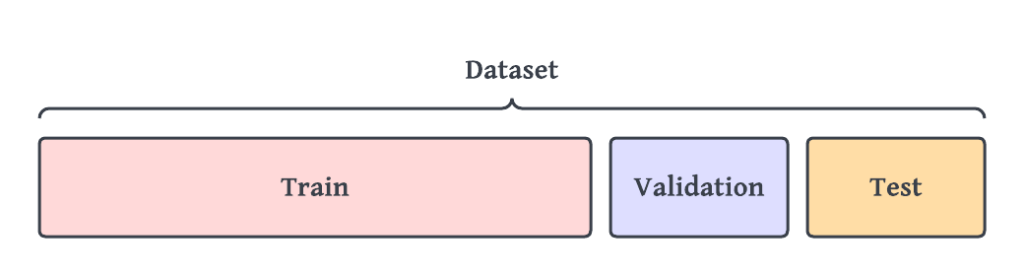
\includegraphics[width=0.5\textwidth]{images/train_test_val.png}
    \caption{Training, Testing, and Validation Sets}
    \end{figure}


The goal of machine learning algorithms is to produce effective prediction models by extracting information from available data. Any machine learning study's broad framework may be summed up as follows.
A dataset containing current data on the issue under study is the first step in any machine learning investigation. Next, the data is divided into three subsets: the test set, the validation set, and the training set. After that, the training data is used in some way to create a machine learning model. To create a mathematical model that represents the training set, the machine learning algorithm examines the data in this phase, which is known as "learning." The performance of this model is then assessed by testing it on the validation set.
\textbf{If the performance levels that are obtained at this point are considered unacceptable, the learning process is repeated to modify the algorithm parameters and revise the model.}
A defined acceptable threshold for validation performance is reached, and then the model is assessed on the test set. The outcomes produced here show the model's ultimate score and cannot be altered further. 

Important things to keep in mind while arranging data for test sets are that:
\begin {itemize}
\item The ML algorithm is built using training data. Information is sent to analysts, who then search for predicted outputs that match. The import must meet all requirements and be of an adequate amount. It is essential to employ unseen values during validation. Here, ML designers may assess the predictive accuracy of the new model thanks to the additional inputs and outputs.
\item Extensive volumes of validation data might lead to overfitting.
\item Test records need to stay untagged, however, supervised machine learning techniques utilize a tag or classifier to identify training data. Results may exhibit anomalies if the ML model can identify a common reference based on the same data labels.
\end{itemize}

\subsection{Training Set}

The training set is used to train the machine learning algorithm. The method generalizes to correctly reply to all potential inputs based on a training set of examples with the right replies (targets) supplied. Based on sample input-output pairs, the machine learning algorithm is charged with learning a function that translates an input to an output. 

\begin{itemize}
    \item The information in a training set needs to be relevant to the task the algorithm is completing for it to provide reliable predictions. 
\item Only when the training sets are relevant can machine learning models provide reliable predictions. This may be compared to training a model to interpret car registration only based on weather data.
\item A training set's data must be representative of every characteristic the model is expected to predict.
\item A training set's data must have the same characteristics. A user training model to identify names and street addresses using data that occasionally contains a gender would be one example. 

\end{itemize}


\subsection{Validation Set}

The validation set is used to calculate the ML model's accuracy. Users check that the new data classification is accurate and produces expected results throughout this step. Validation sets are composed of objective inputs and anticipated outcomes that are intended to verify the model's functionality and efficacy. During this stage, cross-validation (CV) techniques are used. There are several forms of CV, but they all work to guarantee stability by projecting the performance of a prediction model.
Fine-tuning and resampling need several iterations. Regardless of the approach, the goal of these verification procedures is to evaluate the outcomes and compare them to other sources of information. The variables used to regulate the process as a whole or the hyperparameters, can also be changed.

\begin{itemize}
    \item  The model's hyperparameters are adjusted using the validation set, which is regarded as a component of the model's training. The model receives this data just for assessment purposes; it does not derive any knowledge from it, therefore the evaluation is impartial and objective. 
    \item By stopping model training when the loss of the validation dataset exceeds that of the training dataset, the validation dataset may also be used for regression, lowering variance and bias, for example. Depending on the amount of hyperparameters, this data may represent 10–15\% of the overall data available for the project. Specifically, a larger validation set will yield better results if the model has a high number of hyperparameters. 
\end{itemize}

\begin{figure}[h]
    \centering
    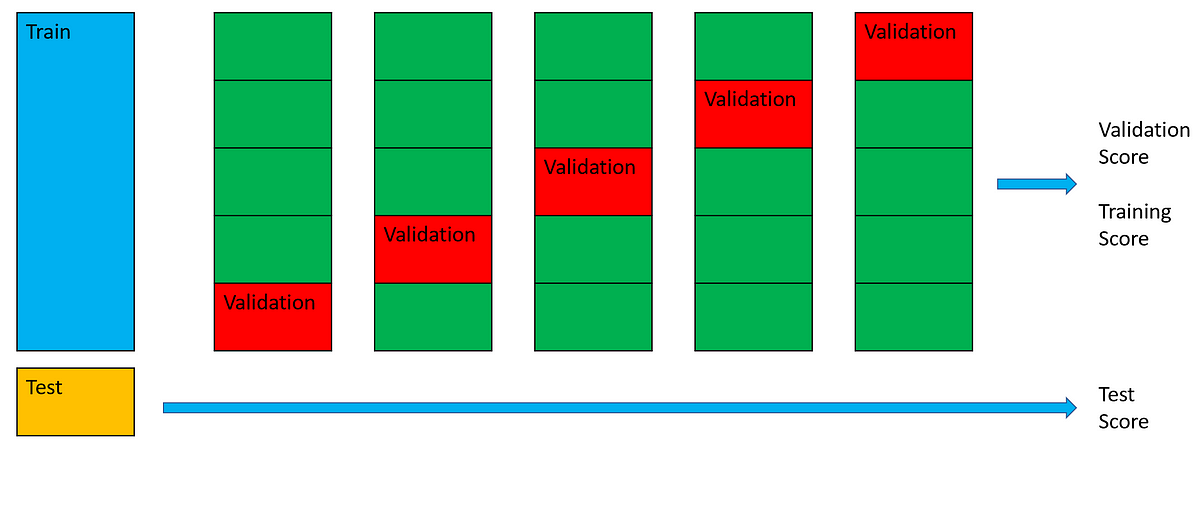
\includegraphics[width=0.5\textwidth]{images/val_set.png}
    \caption{Training, Testing, and Validation Sets}
    \end{figure}

The easiest method for comparing several networks is to assess the error function using data that is separate from the training set, as our objective is to identify the network that performs the best on fresh data. A suitable error function specified about a training data set is minimized to train different networks. Next, the error function of each network is assessed using a separate validation set to compare their performance. The network with the lowest error concerning the validation set is chosen. An example of this process in action is early stopping, in which the training terminates when the error on the validation set increases, selecting the prior model, and the candidate models are essentially repetitions of the same network.


\subsection{Testing Set}

An objective assessment of the model's final fit on the training dataset is provided by the test dataset, which is a sample of data. It offers a benchmark by which the model is assessed. It is only applied when a model has been fully trained with both the train and validation sets. Typically, models are assessed using the test set.

The test set is used to mimic the models' genuine performance in the wild after we have utilized the validation set to identify the method and parameter choices that we might want to use in production. It is the last stage in assessing how well our model performs with unknown data.

\begin{itemize}
    \item **Under no circumstances should we choose a model based on the performance of the test set.**
    \item Overfitting occurs when we look at our test set performance in advance, which might lead to inaccurate performance expectations in real-world scenarios. It needs to be examined as the last kind of assessment, following the identification of the optimal model using the validation set.
\end{itemize}


\begin{figure}[h]
    \centering
    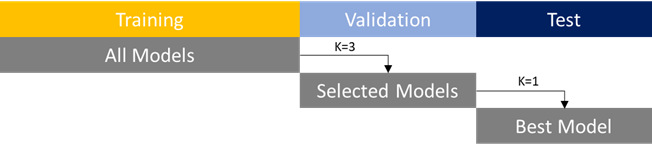
\includegraphics[width=0.5\textwidth]{images/test.png}
    \caption{Training, Testing, and Validation Sets}
    \end{figure}


    A well-structured dataset containing a variety of data for situations that the model is likely to encounter in practice is often utilized as the testing set. A model is said to be overfitting if its accuracy on training data is higher than its accuracy on testing data. This data represents around 10–20\% of all the data that is available for the specified job. Validation and testing may overlap to some extent. Every step demonstrates how the machine learning model will perform in a real-world setting after testing.

    An ideal ratio does not exist when dividing a dataset. The model will pick up rules from the provided data if it is distributed appropriately. Putting most of the data that has been gathered into the training set is the main recommendation. The data must also be shuffled before being separated. Although, this is not always true for time-series datasets. There are different splitting methods available for that purpose.
    
    Both the model and the dataset's sample count determine the optimal split ratio. It takes a bigger validation set to optimize the model the more hyperparameters there are. A smaller dataset, however, can be utilized to verify the model if there are few or no hyperparameters. We can definitely minimize the size of the validation set for models with few or no hyperparameters since they are easier to validate and modify. However, if the model has a lot of hyperparameters, we would still want a big validation set.
    
    
    It is important to be aware of common problems that might have a considerable impact on the performance of the model while implementing machine learning algorithms which are overfitting and underfitting.
    
    \subsection{Overfitting}

Overfitting occurs when a model is too complicated for the training data, especially if it is noisy. Possible solutions are:

\begin{itemize}
    \item Simplify the model by using fewer parameters (e.g., a linear model)
\item Minimizing the number of attributes in the training data
\item Gathering more data
\item Reducing noise (removing errors and outliers)
\end{itemize}


Regularization is the process of limiting a model to reduce overfitting and simplify it. For instance, a linear model could contain two parameters: $\theta_{0}$ and $\theta_{1}$. The learning algorithm can adjust the height ($\theta_{0}$) and slope ($\theta_{1}$) of the line to better fit the training data. If $\theta_{1} = 0$, the algorithm had only have one degree of freedom, it would have difficulty fitting the data appropriately. It would only be able to shift the line up or down to come as near to the training cases as possible, resulting in a mean value. Allowing the algorithm to change $\theta_{1}$ while limiting its size results in a learning method with one to two degrees of freedom. The model will be simpler than with two degrees of freedom, although more complex than with one. To provide good generalizability, the model should strike a compromise between perfectly fitting the training data and being simple.

\subsection{Underfitting}
Underfitting, as one can anticipate, is the reverse of overfitting and happens when your model is too easy to use to understand the underlying structure of the data. For instance, a linear model of life happiness is likely to underfit since, even with training samples, the reality is just too complicated for the model to accurately predict.
To address this issue, the primary alternatives are:
\begin{itemize}
\item Opting for a more robust model with more parameters
\item Introducing improved features (feature engineering) into the learning algorithm
\item Minimizing the model's restrictions, such as lowering the regularization hyperparameter
\end{itemize}

Finally, accurate identification as well as usage of training, validation, and testing sets are essential for the success of machine learning projects. Experts are capable of creating stronger, more reliable, and generalizable models if they are mindful of the goal of each dataset and avoid traps like overfitting and underfitting.
\section{Model Replication of the Hill Climbing Algorithm}
This section presents a replication of the Hill Climbing Algorithm as implemented by Alvi et al., with the accompanying notebook detailing the process. The algorithm is employed to estimate the fundamental components of Hidden Markov Models (HMMs): Initial Probabilities (start state likelihoods), Transition Matrix (state-to-state transition probabilities), and Emission Probabilities (observation likelihoods given states). 

\subsection{Initial Probabilities}
\begin{tabular}{lr}
\toprule
 & 0 \\
\midrule
0 & 0.513109 \\
1 & 0.237780 \\
2 & 0.249111 \\
\bottomrule
\end{tabular}

\subsection{Transition Matrix}
\begin{tabular}{lrrr}
\toprule
 & 0 & 1 & 2 \\
\midrule
0 & 0.586389 & 0.330278 & 0.083333 \\
1 & 0.013318 & 0.624335 & 0.362347 \\
2 & 0.352194 & 0.018419 & 0.629387 \\
\bottomrule
\end{tabular}

\subsection{Emission Probabilities}
\begin{tabular}{lrr}
\toprule
 & 0 & 1 \\
\midrule
0 & 0.820043 & 0.179957 \\
1 & 0.200328 & 0.799672 \\
2 & 0.764277 & 0.235723 \\
\bottomrule
\end{tabular}



\section{Model Validation Process}
The study adequately presents the practical differences between training, testing and validation processes, albeit with usage of unprofessional language like capitalized words and exclamation marks. 

It proposes algorithmic performance evaluation through trading simulations, initially focusing on a single oil share. Upon achieving satisfactory validation results, the model is tested. The validation process helps in model adjustment in case of high error rates, maybe necessitating a  re-initialization of the Hill Climbing method for Bayesian model learning. The paper categorically mentions that testing is advised only after attaining satisfactory validation performance, maintaining methodological integrity and preventing data leakage.
\section{Visualisation Techniques}
\subsection{Heatmaps}
A Markov transition matrix, which captures the probabilities of transitioning from one state to another in a Markov chain, can be effectively visualized as a heatmap to reveal underlying patterns and structures in the data. Each entry in the matrix corresponds to the probability of moving from a given state to another, and when represented as a heatmap, these probabilities are depicted as varying intensities of color. This visualization allows for the immediate identification of prominent transitions (high probability values), which appear as brighter or more intense areas, while less likely transitions are represented by darker or subdued tones. \cite{genc2019optimal} 


\begin{figure}[H]
    \centering
    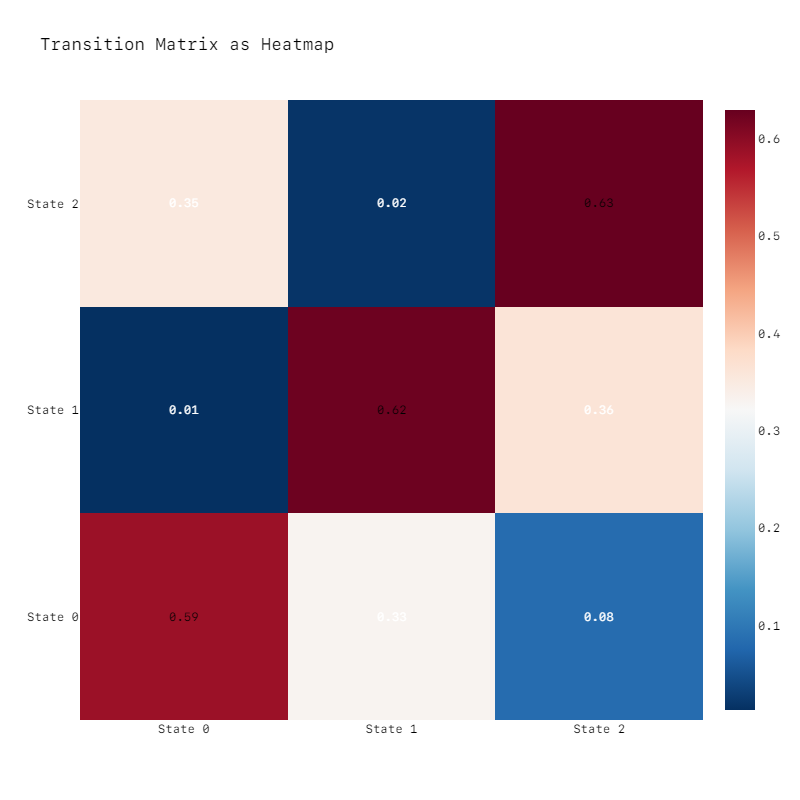
\includegraphics[width=0.5\textwidth]{images/heatmap.png}
    \caption{Heatmap of a Markov transition matrix}
    \label{fig:heatmap}
\end{figure}

\subsection{Directed Acyclic Graphs}
A Bayesian network, which represents a set of variables and their conditional dependencies via a probabilistic graphical model, can be effectively visualized as a Directed Acyclic Graph (DAG). In this representation, each node in the DAG corresponds to a variable, and directed edges between nodes signify the conditional dependencies, where an edge from node A to node B indicates that B is conditionally dependent on A. The acyclic nature of the graph ensures that there are no feedback loops, thereby maintaining the probabilistic consistency of the model. 


\begin{figure}[H]
    \centering
    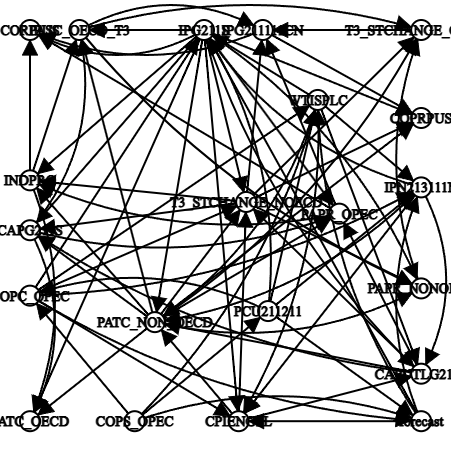
\includegraphics[width=0.5\textwidth]{images/graph.png}
    \caption{Heatmap of a Markov transition matrix}
    \label{fig:heatmap}
\end{figure}


\section{Predictive Accuracy of the Model}
\section{Contribution of the Study}
\printbibliography

\end{document}